%This part describes the implementation of the HELIOS concept
\chapter{The Solenoid}
\label{sol}
The magnet used in HELIOS is a superconducting solenoid from a decommissioned Siemens model OR63  Magnetic Resonance Imaging (MRI) scanner.  The solenoid had previously been used as a research MRI at the Max Planck Institute for Biological Cybernetics in T\"ubingen, Germany.  The OR63 solenoid is a prototype model similar to the OR64 production  model, going under the trade name 3T MAGNETOM Trio, a whole-body medical diagnostic scanner.  When used as medical diagnostic, the MRI scanner produces an RF perturbation to the otherwise homogeneous magnetic field of the solenoid.  However, for the purposes of HELIOS, the solenoid field is kept at a fixed value and left unperturbed. % (``persistence mode'').
The HELIOS solenoid was delivered to Argonne and installed in the then-named General Purpose Area in December, 2006.

\section{Vacuum Chamber}

\begin{figure}%
\centering
%%\includegraphics[width=\columnwidth,height=0.4\textheight,keepaspectratio]{MRI_interior}\\
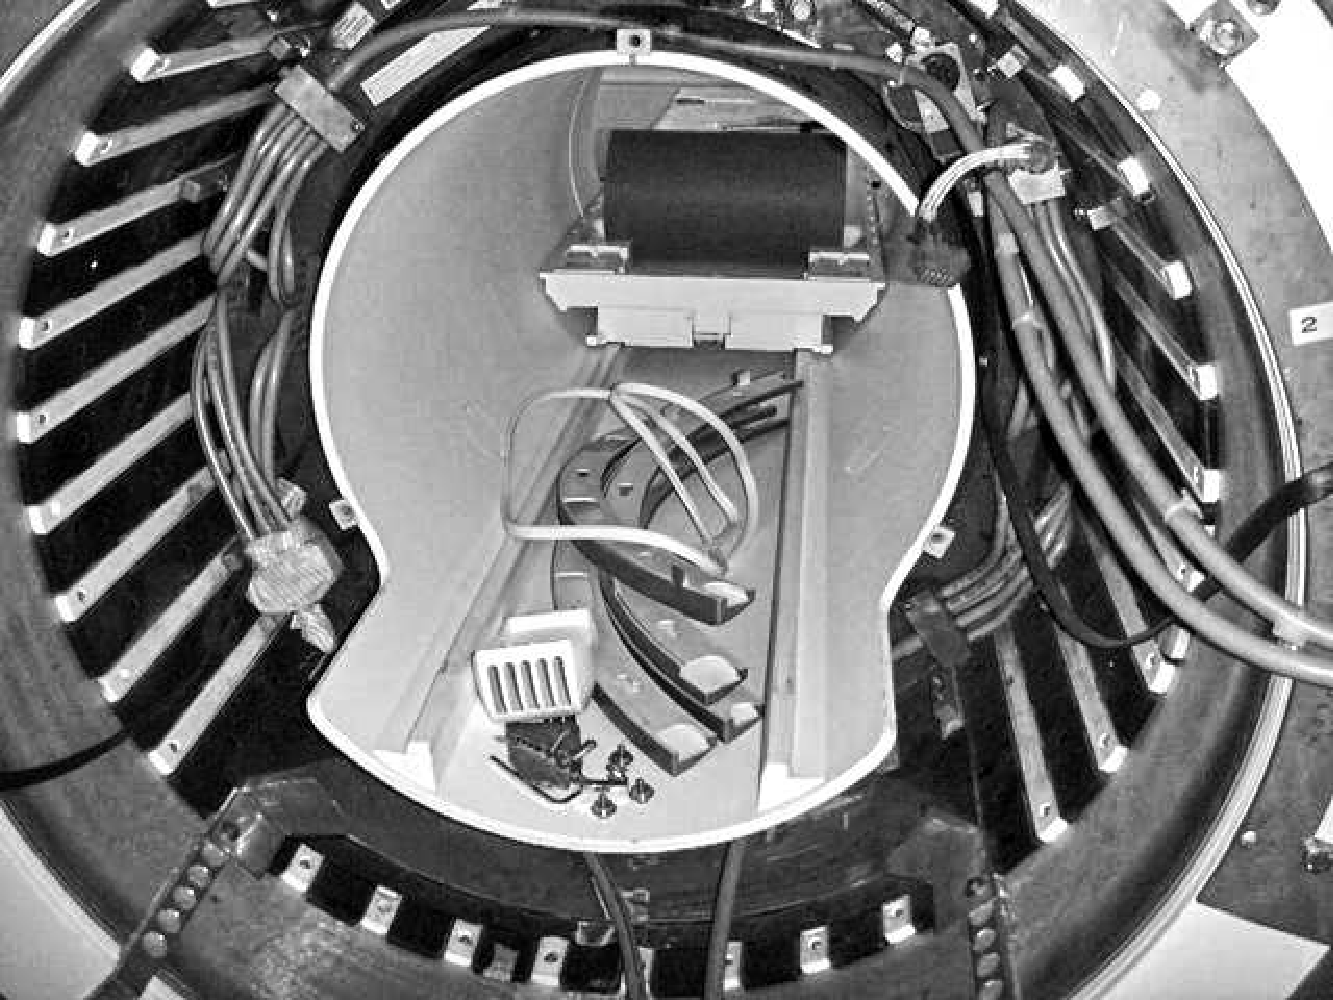
\includegraphics[width=.45\columnwidth,height=0.4\textheight,keepaspectratio]{PICT0036_bw}~
%\includegraphics[width=.45\columnwidth,height=0.4\textheight,keepaspectratio]{dsc00997}%
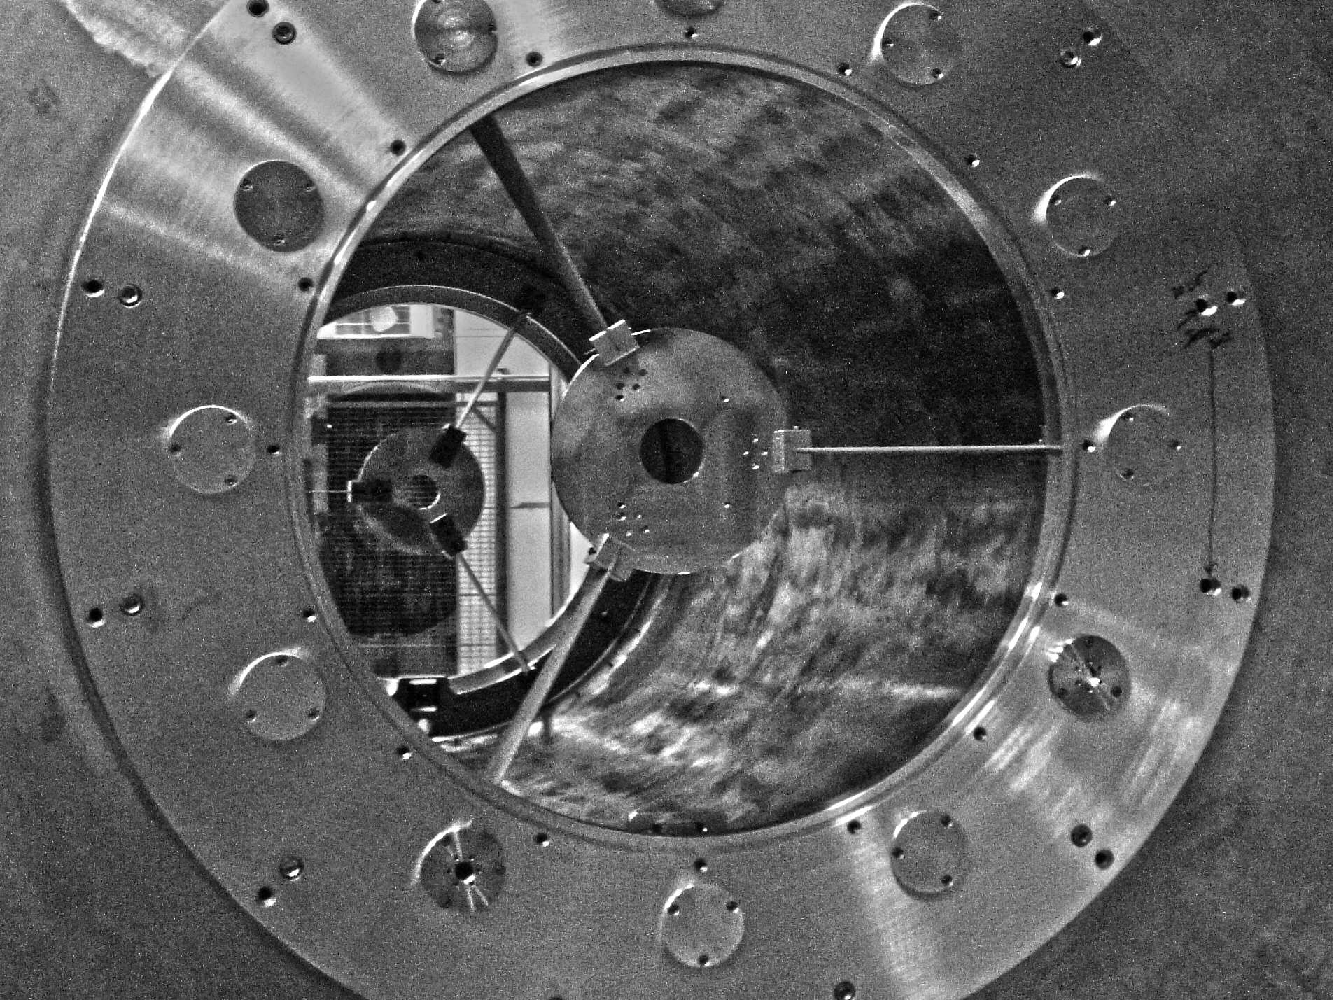
\includegraphics[width=.45\columnwidth,height=0.4\textheight,keepaspectratio]{dsc01224}%
\caption[The ``Patient End'' of the HELIOS solenoid before and after conversion to a spectrometer]{The ``Patient End'' of the HELIOS solenoid before and after conversion to a spectrometer; (left) showing MRI scanning hardware, and (right) showing the large adapter flange and alignment ``spider''. Photo (left) by B.~B.\ Back, \photodate\formatdate{6}{11}{2006} }%
\label{MRI}%
\end{figure}

For use as a nuclear spectrometer, the hardware associated with MRI scanning had to be removed (see Fig.~\ref{MRI}).  Stripped of scanning hardware, the interior diameter of the solenoid bore is 92.5\,cm and 234.7\,cm in length.  Based on sonic measurements, the solenoid wall was determined to be 5.3\,mm thick.  With the interior hardware removed, the bore-surface of the solenoid was polished to make it suitable as a vacuum chamber.  The ends of the solenoid featured square-faced mounting faces for annular field shims%called --- look up in users manual
.  These mounting faces permitted the entire solenoid volume to be converted to a vacuum vessel by sealing the ends of the bore with large-opening aluminum adapter flanges% mounted to either end of the solenoid
.

Each adapter flange has an opening diameter of 71.12\,cm and features twelve 4.45\,cm diameter feedthroughs.  These feedthroughs are used for a variety of functions as described throughout the following chapters, including detector signals.  An additional removable flange reduces the opening to mate with a 20\,cm diameter beam-line pipe.  This flange features four 16.51\,cm diameter feedthroughs.  A 20\,cm beam pipe is used for HELIOS instead of the ATLAS-standard 10\,cm beam pipe to aid in vacuum pumping.  All of the hardware in the immediate vicinity of the magnet is constructed from non-\-magnetic materials---primarily aluminum alloys and 316 stainless steel.  A photograph of the HELIOS solenoid, fully converted for use as a spectrometer, appears in Fig.~\ref{solenoid}.

\begin{figure}
\centering
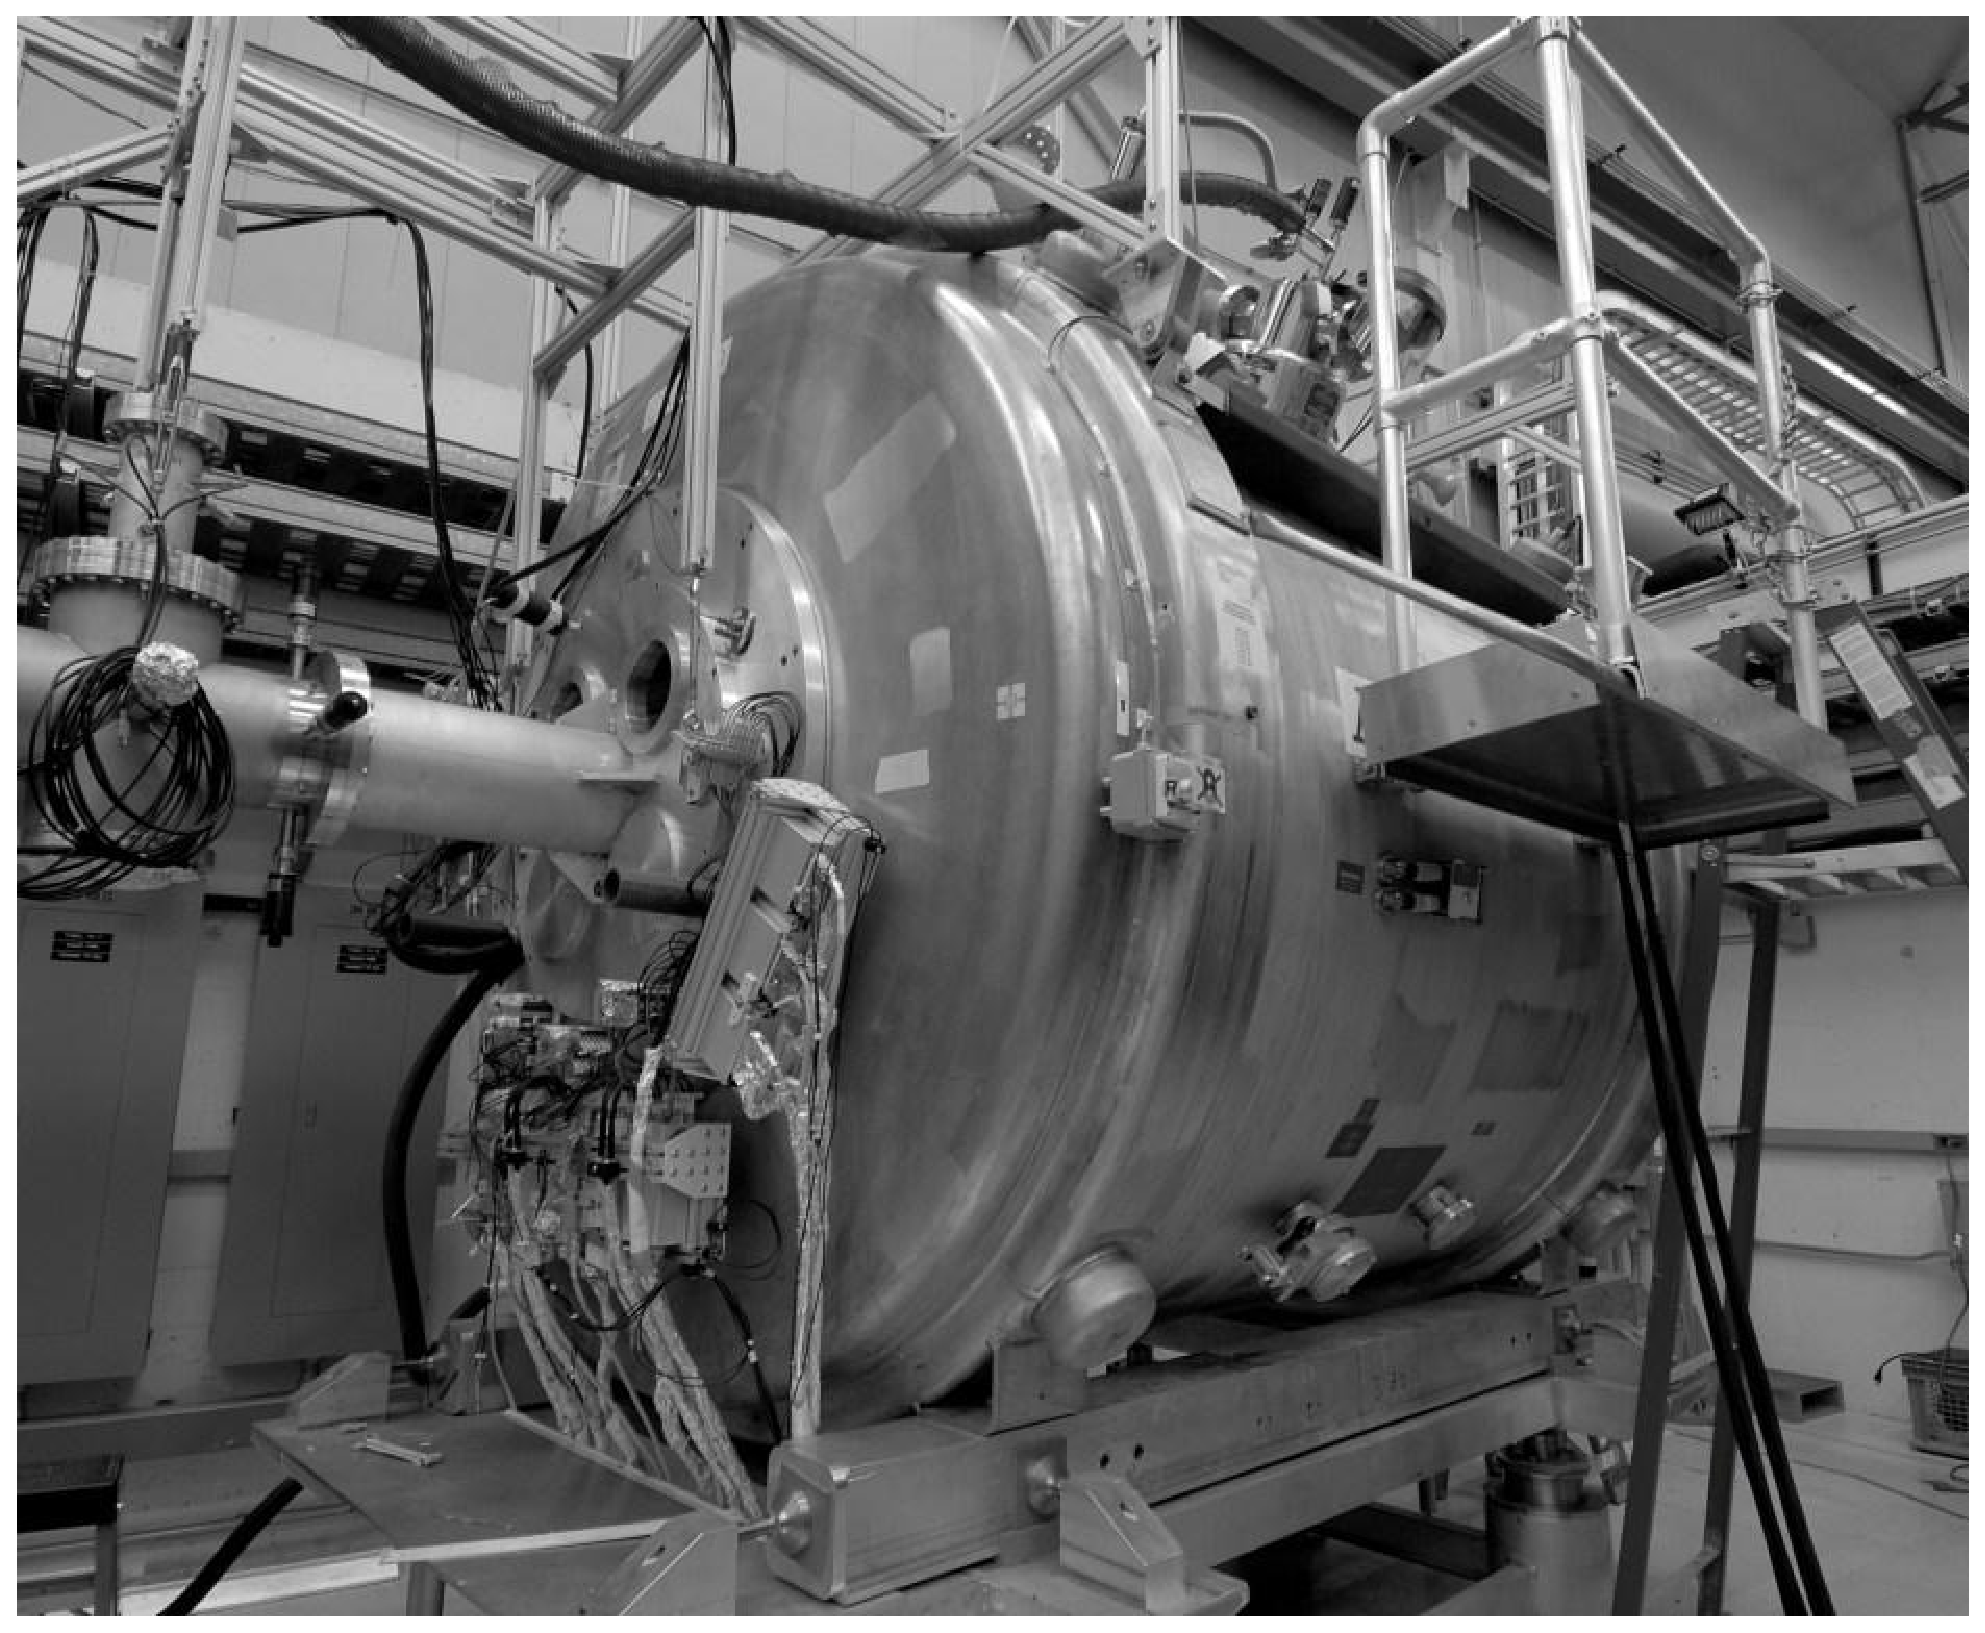
\includegraphics[width=\linewidth,height=0.4\textheight,keepaspectratio]{../NIM_Paper/Figures/DSC_0792_compressed}
\caption[The HELIOS spectrometer as installed at the ATLAS accelerator]{The HELIOS spectrometer as installed at the ATLAS accelerator.  Beam enters from left.  The preamplifers are mounted to the bottom and lower right-hand side of the 115\,cm diameter sealing flange.  Photo by A.~H. Wuosmaa, \photodate\formatdate{15}{3}{2010}.  This figure also appears in Ref.~\cite{Lighthall_2010}.}
\label{solenoid}
\end{figure}

\section{Field Map}
Particle trajectories calculated analytically, such as those presented in Chapt.~\ref{HELIOS_Concept}, assume a purely axial, uniform magnetic field.  Such a field is produced by an ``ideal'' solenoid of infinite length.  However, a realistic solenoid of finite length will produce a magnetic field with systematic non-\-uni\-for\-mi\-ties.  To account for the effects of such non-uniformities, the non-uniformities can be modeled, as in Ref.~\cite{Wuosmaa_2003}, or the field map of an existing magnet can be used, as in Ref.~\cite{Wuosmaa_2007}.  In order to assess and characterize the HELIOS solenoid, a map of the magnetic field was made in October, 2007.
%\subsection{Measurement}
\subsection{Equipment}
The components of the magnetic field were measured using an F.~W. Bell Model ZOA73-3208 three-axis Hall probe.  The probe was read out via an F.W. Bell Series 9900 Gaussmeter.  The probe consisted of an aluminum rod, 20\,cm long and 0.79\,cm in diameter, mounted in a plastic handle with the Hall probe sensors near the tip of the rod (see Fig.~\ref{probe}).  The Hall plates within the probe had a stated mutual perpendicularity of $\pm 2^\circ$. Both pieces of hardware were used in a previous application.  

Measurements were read out passively with the gaussmeter in ``master'' mode by a purpose-written program using LabVIEW\texttrademark.  Throughout the field measurements the gaussmeter was kept in a region of low magnetic flux ($<500$\,$\mu$T) while extension cables allowed the probe to be moved throughout the solenoid volume.  The gaussmeter had a stated DC resolution accuracy of $\pm0.035$\%.  For example, 0.01\,$\mu$T (1\,mG) resolution at a field of 300\,$\mu$T (3\,G) and 100\,$\mu$T (10\,G) resolution at 3.0\,T.  The probe was calibrated for probe and circuit offset errors by placing the probe in the gausmeter's 80\,dB attenuation shielded ``zero gauss'' chamber.
 
After considering a variety of probe jig designs, such as an articulating arm on a cart, it was decided to mount a rotating probe jig to the flange faces of the solenoid. %, as shown in Fig.~\ref{MRI}.
  This approach was chosen to provide reproducibility in measurement position by having the probe jig mounted to the solenoid and to take advantage of the cylindrical symmetry of the solenoid.   In this configuration, the three measured components corresponded to the axial ($\vec{\mathscr{B}}\cdot\hat{z}$), radial ($\vec{\mathscr{B}}\cdot\hat{\rho}$), and azimuthal ($\vec{\mathscr{B}}\cdot\hat{\phi}$) components of the magnetic field.
\begin{figure}%
\begin{center}
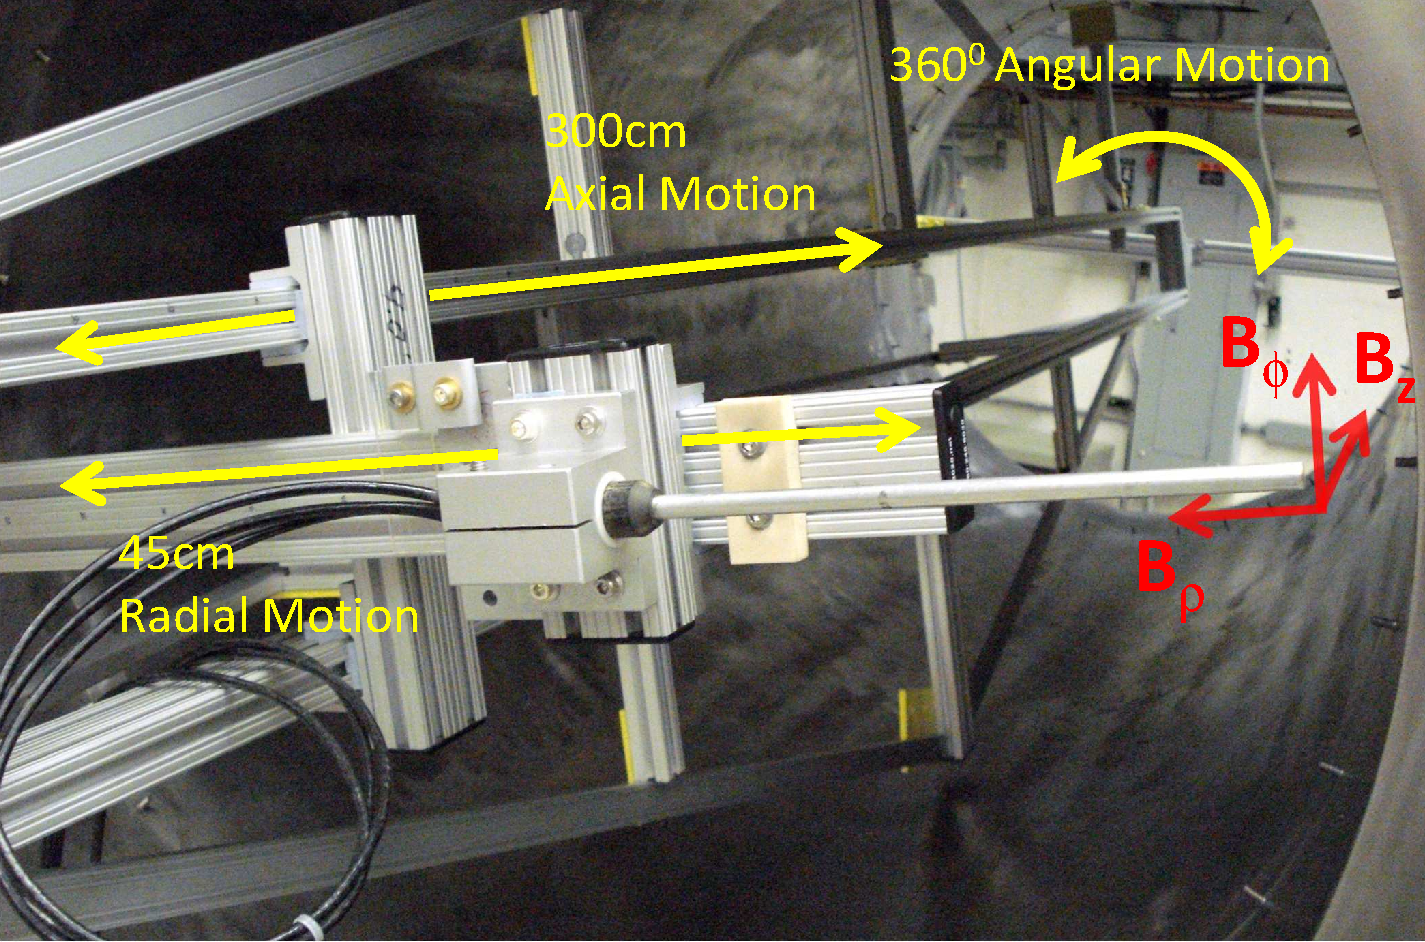
\includegraphics[width=\columnwidth, height=0.38\textheight,keepaspectratio]{probe3}%	
\end{center}
\caption[Hall probe mounted in the field mapping jig within the solenoid volume]{Hall probe mounted in the field mapping jig within the solenoid volume.  The probe jig is design so that the tip of the Hall probe rotates along a path concentric with the solenoid bore At each combination of axial position and angle, the probe translates along the radius of the solenoid.}%
\label{probe}%
\end{figure}

\subsection{Alignment}
Two parallel rails ran the length of the solenoid axis, allowing the probe to move on linear bearings over a range of $-175.85\leq z \leq +114.15$\,cm, relative to the mechanical center of the solenoid (the solenoid itself covering a range of $\pm117.35$\,cm).  The axial rails of the probe jig straddled the mechanical axis of the solenoid such that the probe could travel along a radial path, thus sampling the field along the solenoid axis ($\rho = 0$).  Due to the great length of the axial rails, the probe jig had to be structurally reinforced.  Trusses were added to the axial rails to increase their rigidity and minimize sagging.

The field probe was oriented with the body of the probe aligned radially, with the tip of the probe pointing outward.  With the trusses in place, the probe was aligned to rotate in a circular path, concentric with the rim of the flange faces to within 0.5\,mm.  The radial and axial rails were graduated every 5\,cm~$\pm 0.5$\,mm for linear measurement reproducibility.  Each downstream end of the magnet (shown in Fig.~\ref{MRI}) had screws protruding from the solenoid bore every 10$^\circ$.  These screws were used as reference points (and anchors) for measurements made at different rotation angles.

The design iteration shown in Figs.~\ref{MRI} and~\ref{probe} featured two linear bearings connecting the central carriage of the jig to the axial arms.  Measurements made with this configuration showed 100+\,G variations and discontinuities through central region of the solenoid where the field is expected to be uniform.  It was determined that these variation were due to the radial arm of the probe jig pivoting in place.  This design was later upgraded to six anchoring points on the axial rails, keeping the radial arm of the jig rigidly perpendicular to the axial rails.  The reinforcement of the radial arm eliminated the apparent variations in the axial field.

Within the tip of the probe, the Hall plate sensors had to be aligned to the mechanical axes of the solenoid. The method by which the probe was aligned within the jig is illustrated in Fig.~\ref{probe_align}.  The tip of the probe was placed within 1\,cm of center of the solenoid.  Then the probe was then oriented within the jig to maximize the reading on the ``axial'' Hall probe.

\begin{figure}%
\centering
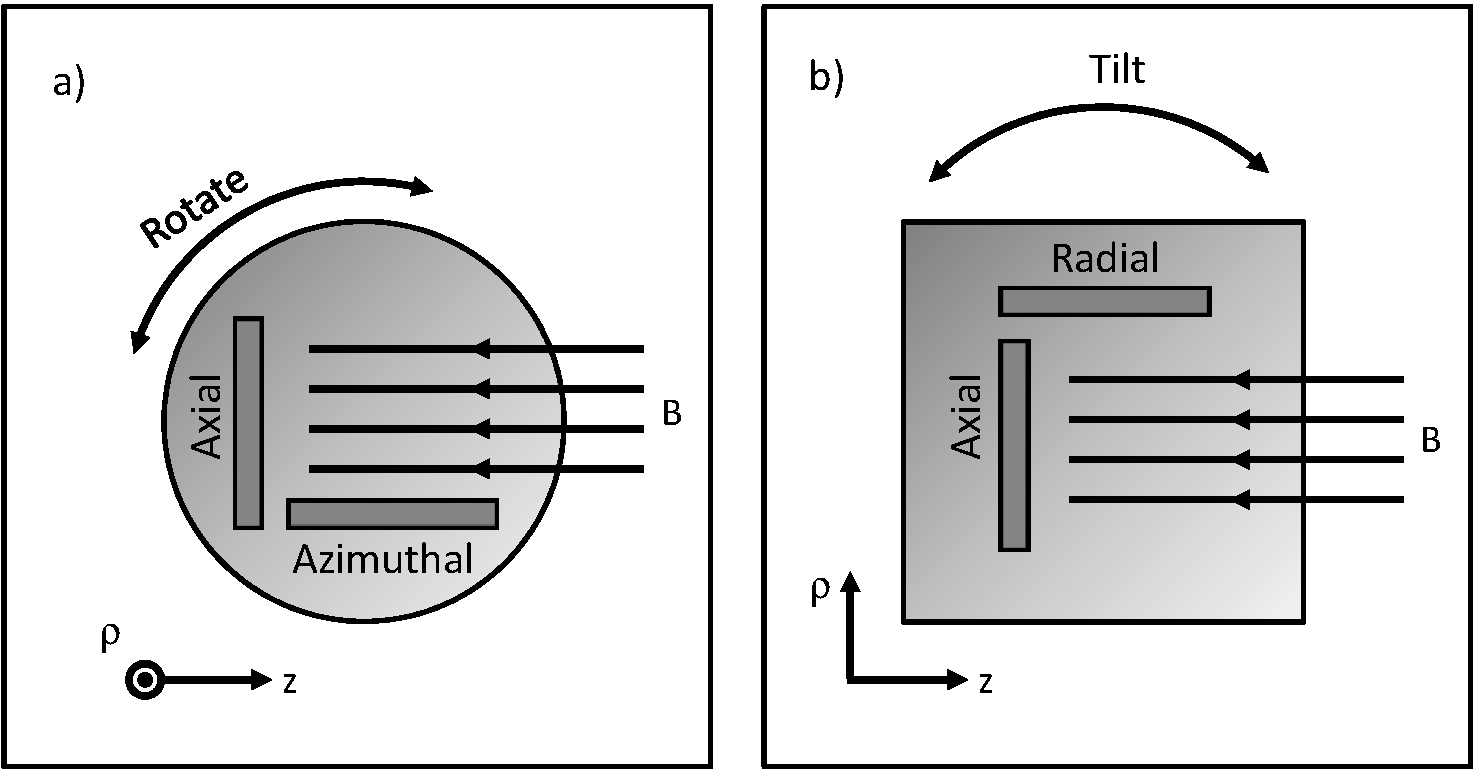
\includegraphics[keepaspectratio,height=0.5\textheight,width=\columnwidth]{probe_align}%
\caption[Illustration of the method of alignment of the 3-axis Hall probe]{Illustration of the method of alignment of the 3-axis Hall probe.  The magnetic field is directed right to left in both figures.  The probe is aligned by a) rotating the probe along its radial axis to minimize the reading in the ``azimuthal'' Hall plate.  Next, b) the probe is tilted in the $\rho$-$z$ plane to minimize the reading in the ``radial'' Hall plate.}%
\label{probe_align}%
\end{figure}

\subsection{Method}
Measurements were carried out by rotating the jig with the probe at fixed $z$ and $\rho$ positions, taking a measurement every 10$^\circ$.  At each $z$ position, this process was repeated at radii every 5\,cm between 0--45\,cm, inclusive.  Thus, each cross section contains 360 data points comprised of 10 concentric circles.  A total of 59 such field cross sections were measured every 5\,cm over a range of nearly 3\,m.  The result is a magnetic field map of 21,240 points inside and outside the solenoid volume with a corresponding average measurement lattice spacing of 4.4\,cm.  An averaged and interpolated version of the field map made up of 410 points appears in Appendix~\ref{field_map_data}.
 
\section{Field Analysis}
Fig.~\ref{map} shows the results of the field mapping.  For each combination of $z$ and $\rho$, the points have been averaged over the 36 angular measurements.  Every other radius set up to $\rho=40$\,cm has been plotted for clarity.  The deviations from uniformity of the magnetic field take the form of systematic variations in the axial and radial field components of the field.    

\begin{figure}%
\centering
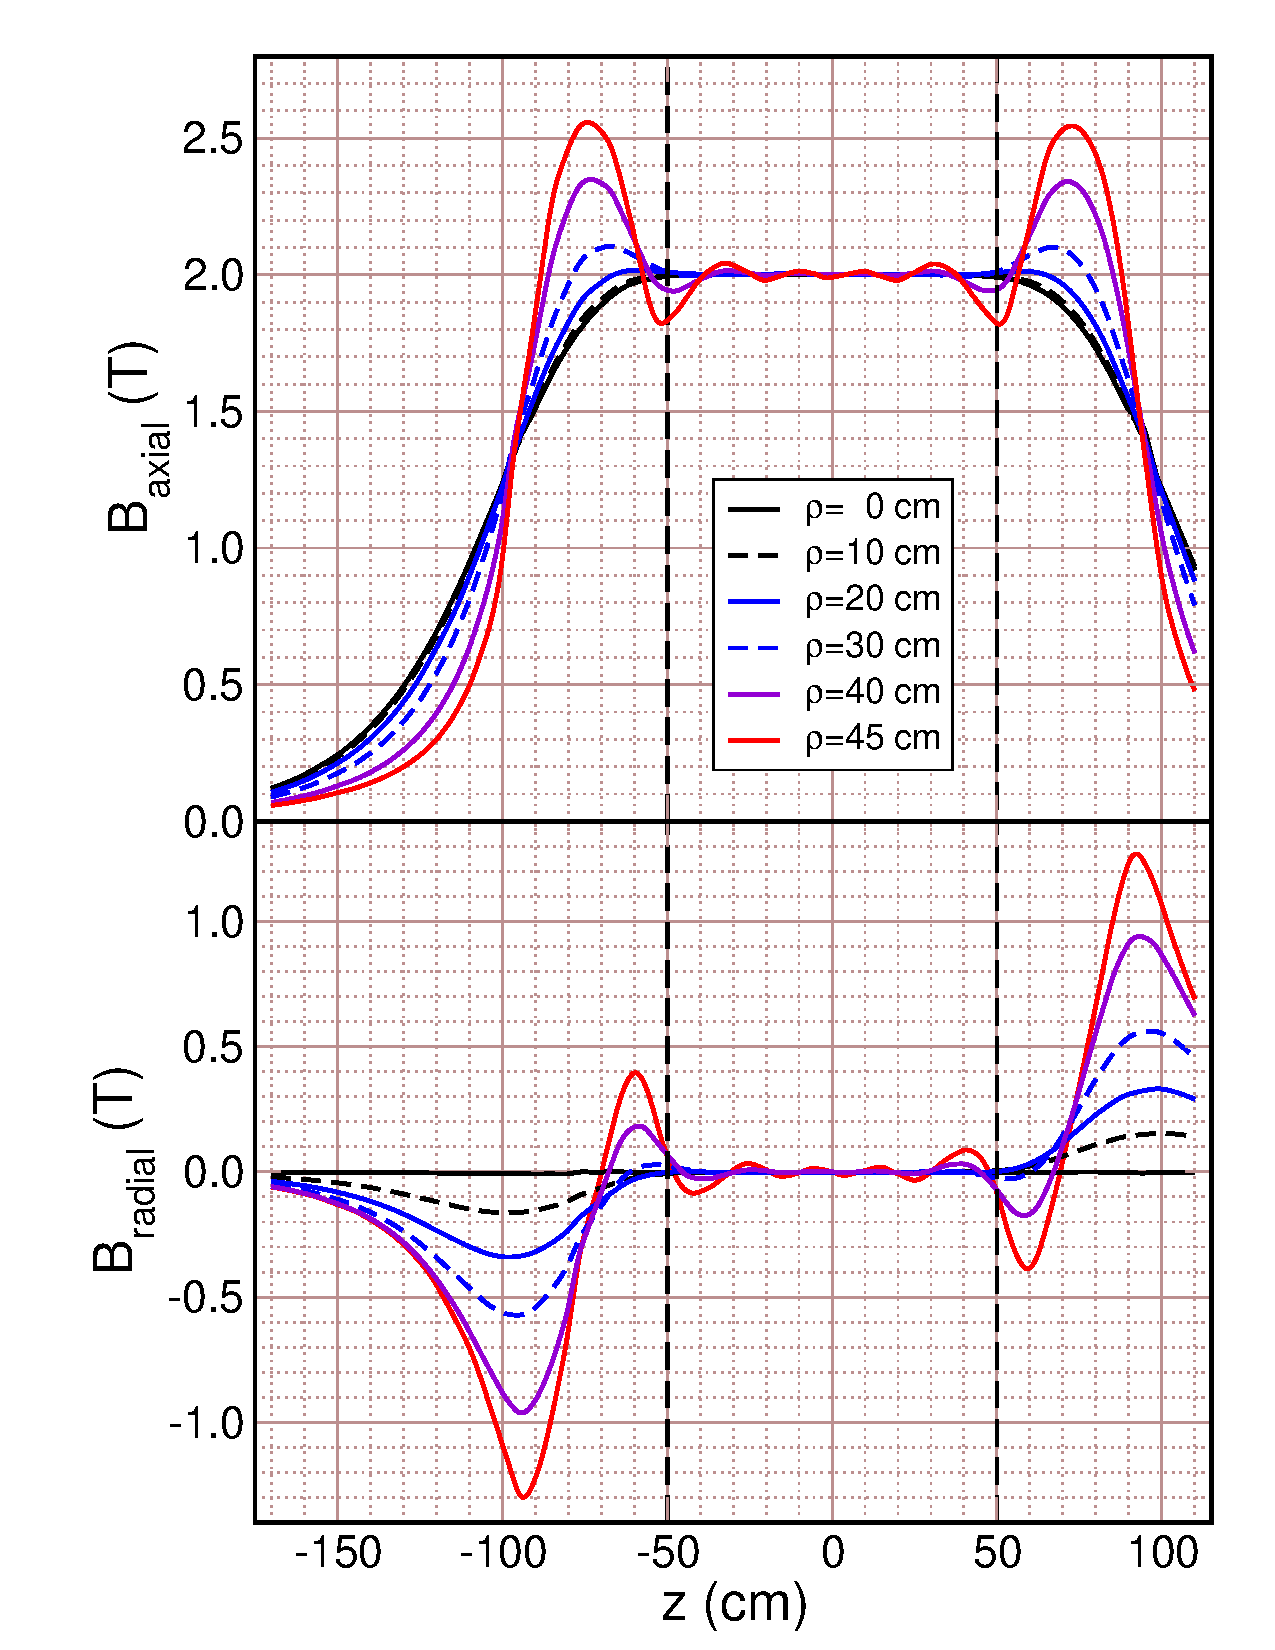
\includegraphics[keepaspectratio,height=0.9\textheight,width=\columnwidth]{field_map_45}%
\caption[Field map of the HELIOS solenoid]{Field map of the HELIOS solenoid.  The axial and radial field components are plotted with a spline fit to the measured values as a function of axial position for five different radii.  The vertical dashed lines indicate the fiducial cylindrical volume.}%
\label{map}%
\end{figure}

\subsection{Gross Structure}
\subsubsection{Axial}
The structure of the magnetic field is consistent with that produced by a 6-coil superconducting solenoid with a 2-coil active shield~\cite{Montgomery_1969}.  This is the structure which is presented schematically in the solenoid service manual.  The effect of these coils is evinced by the 6 peaks and 2 prominent troughs in the $\rho=45$\,cm axial field map in Fig.~\ref{map}.  The axial field is symmetric to within the precision of the measurements about a point offset -0.5\,cm from the mechanical center of the magnet.  This symmetry is demonstrated in Fig.~\ref{axial_reflect}.  The ``kink'' in the axial field at about $z= \pm95$\,cm from the center is consistent with two concentric solenoids with opposite current~\cite{Montgomery_1969}.

\begin{figure}%
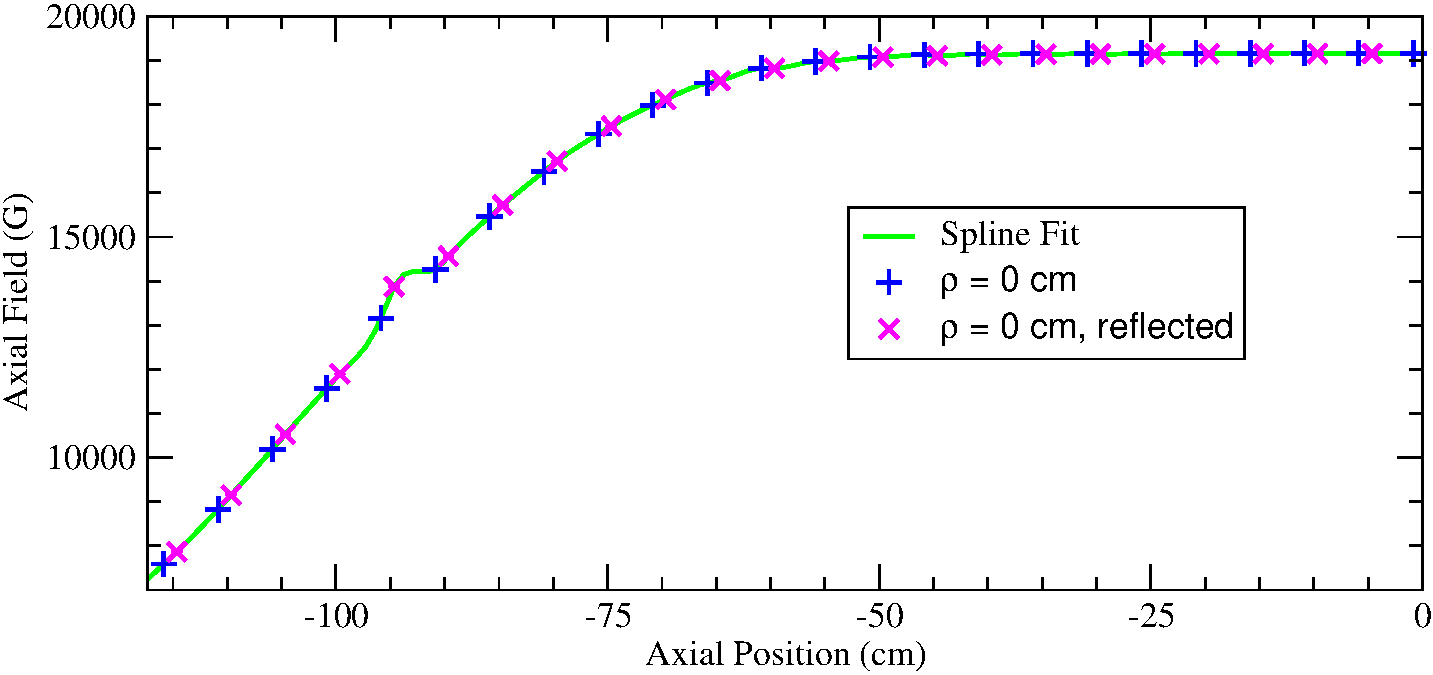
\includegraphics[width=\columnwidth]{axial_fit}%
\caption[Symmetry of the axial field component over the interior of the solenoid]{Symmetry of the axial field component over the interior of the solenoid. The upstream axial field has been reflected about $z=-0.5$\,cm.  The combined points have been fit with a spline fit.  Error bars on position and field are on the order of the line thickness.  }
\label{axial_reflect}%
\end{figure}

On the solenoid axis, the axial field falls to 10\% of its central value at approximately $z= \pm150$\,cm from the center of the magnet and to 0.1\% at approximately $z= \pm230$\,cm from center.  At distances greater than 175\,cm from the center of the magnet, the fringe field is well approximated by an inverse-cubic function ($\mathscr{B}_z\approx 1/z^3$).  The south pole of the average axial magnetic field corresponds to the ``Patient End'' of the solenoid; as shown in Fig.~\ref{MRI}, this end is the downstream end of the solenoid.

\subsubsection{Radial}
Throughout the solenoid, the radial field component is well approximated by a third-order polynomial function of the cylindrical radius $\rho$.
\begin{equation}
\mathscr{B}_\rho=A+B\rho+C\rho^2+D\rho^3
\label{eq:radial}
\end{equation}
  The radial field reaches a maximum absolute value of 63\% of the central field approximately $z= \pm95$\,cm from the center of the magnet at a cylindrical radius of $\rho =45$\,cm, corresponding to the location of the fringe field reducing coils.  

\subsubsection{Tangential}
The ``tangential'' or azimuthal component of the magnetic field ($\vec{\mathscr{B}}\cdot\hat{\phi}$) was  measured to be less than 1.8\% of the total magnetic field and had an average value of 0.32\% of the total magnetic field.  Fig.~\ref{tan_field} shows a representative example of the tangential field, measured at $\rho=15$\,cm.  Included in the plot are fitted projections of both the axial and radial fields.  The results of such fits at all radii indicate that the ``azimuthal'' Hall plate sensor was $0.07^\circ \pm 0.02^\circ$ away from perpendicular, relative to the ``axial'' sensor, and $1.31^\circ \pm 0.14^\circ$ away from perpendicular, relative to the ``radial'' sensor.  The residual azimuthal component is asystematic and structureless, consistent with zero.

\begin{figure}%
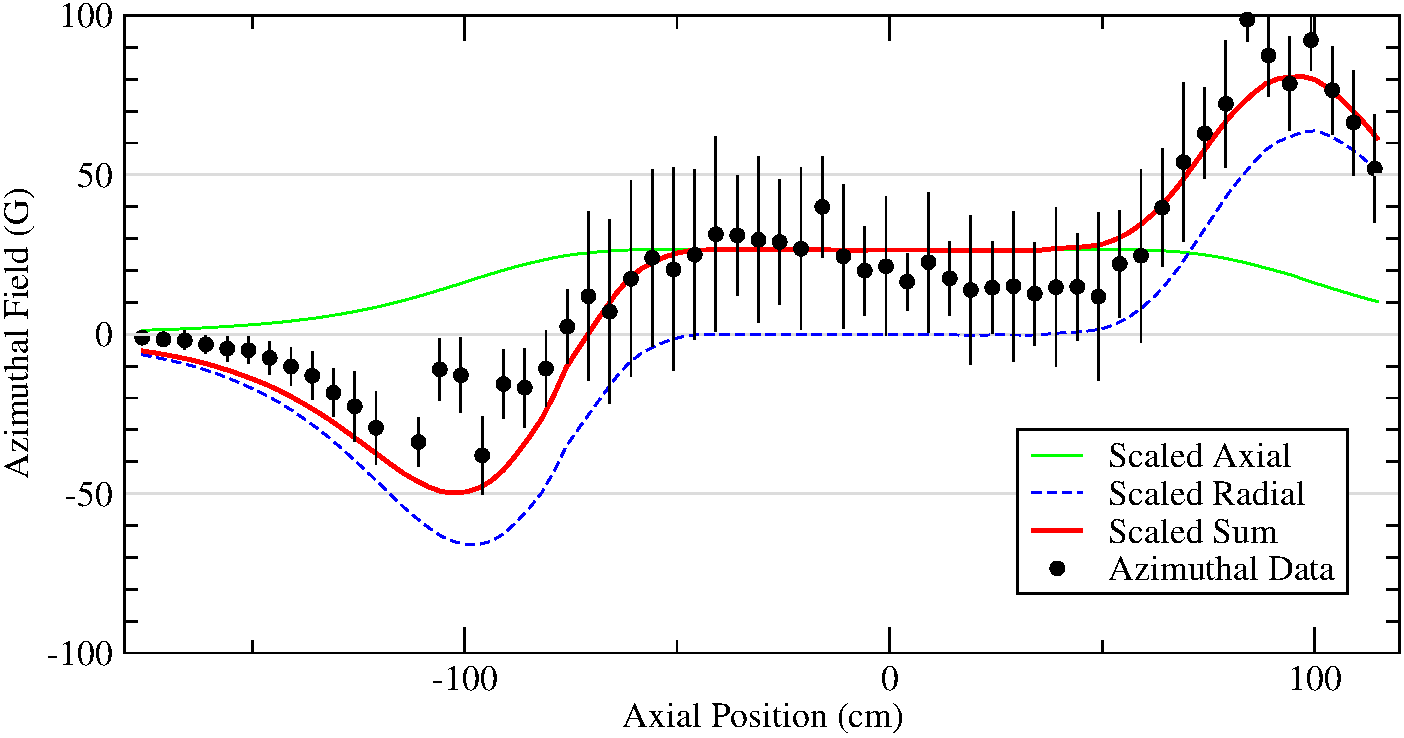
\includegraphics[width=\columnwidth]{r15_tan}%
\caption[Azimuthal  field component at $\rho=15$\,cm with projected fit of the other field components]{Azimuthal  field component at $\rho=15$\,cm with projected fits of the other field components.  Error bars of 1\,$\sigma$ are shown.  Nearly all of the points are within 1\,$\sigma$ of the scaled sum, indicating the ``azimuthal field'' is consistent with zero.}%
\label{tan_field}%
\end{figure}

\subsubsection{Uniformity}

The magnetic field is homogeneous and purely axial in a spherical field region about the geometric center of the solenoid, referred to as the Diameter Spherical Volume (DSV).  For medical purposes, similar magnets are guaranteed to have a homogeneous region (``Field of View'') 40\,cm in diameter.  
In this region, the measured variation in the magnetic field is less than the stated measurement uncertainty (0.035\%) and is consistent with zero.  In a 90\,cm DSV, which extends to the solenoid bore, the mean absolute field non-uniformity is slightly higher at 0.05\%.  
The absolute field non-uniformity increases to a maximum of 3.1\% within a central cylindrical volume 1\,m long and 40\,cm in radius.  Section \ref{simulation} describes how these characteristics define the fiducial volume of the spectrometer.

\subsection{Fine Structure}
A detailed analysis of the field map revealed systematic azimuthal variations in the measured radial field components.  An example such variations is shown in Fig.~\ref{sine_fit}.  Variations of this kind are consistent with an offset between the rotational axis of the field mapping jig and the magnetic field axis.  Fig.~\ref{map_off} illustrates how these variations may arise.  If the probe is rotated along a circular path which is offset from the magnetic field axis, a range of magnetic equipotentials are sampled.  The result would be a sinusoidal variation in the measured magnetic field as shown in Fig.~\ref{sine_fit}.

\begin{figure}%
\centering
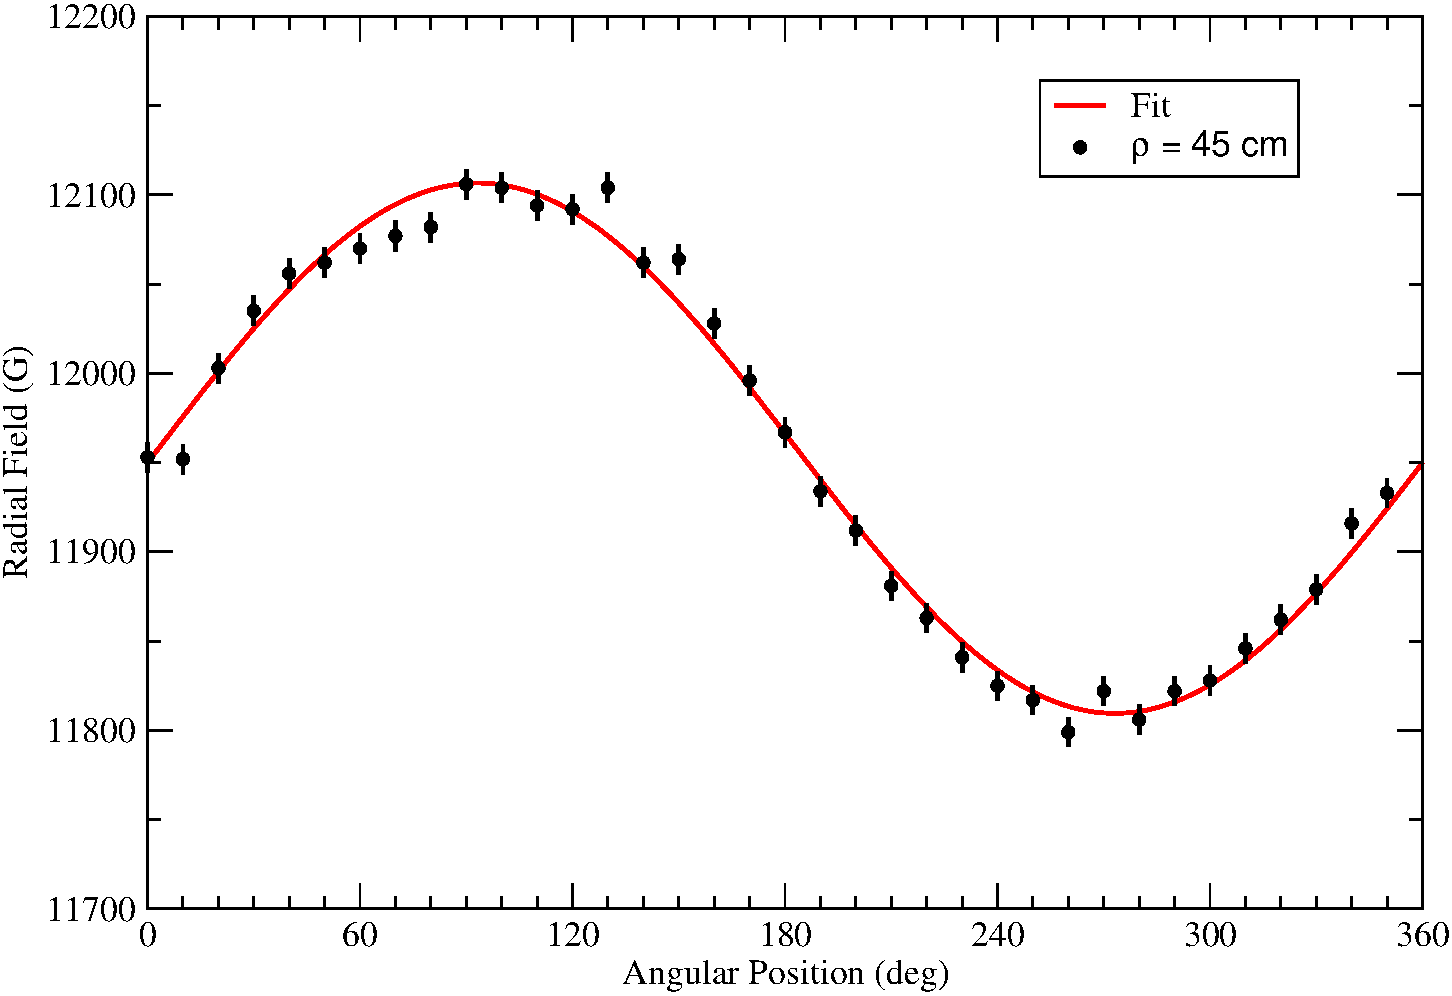
\includegraphics[width=\columnwidth,height=0.4\textheight,keepaspectratio]{sine_fit}%
\caption[Measured azimuthal variation in the radial field component at $z=94.15$\,cm, $\rho=45$\,cm]{Measured azimuthal variation in the radial field component at $z=94.15$\,cm, $\rho=45$\,cm.   $\pm 0.035$\% error bars are shown.  The data have a fluctuation of $\pm 63$\,G about the mean.  The line is a sine cure fit to the data ($\chi^2/\textrm{dof}=1.98$).}%
\label{sine_fit}%
\end{figure}

\begin{figure}%
\centering
\fbox{
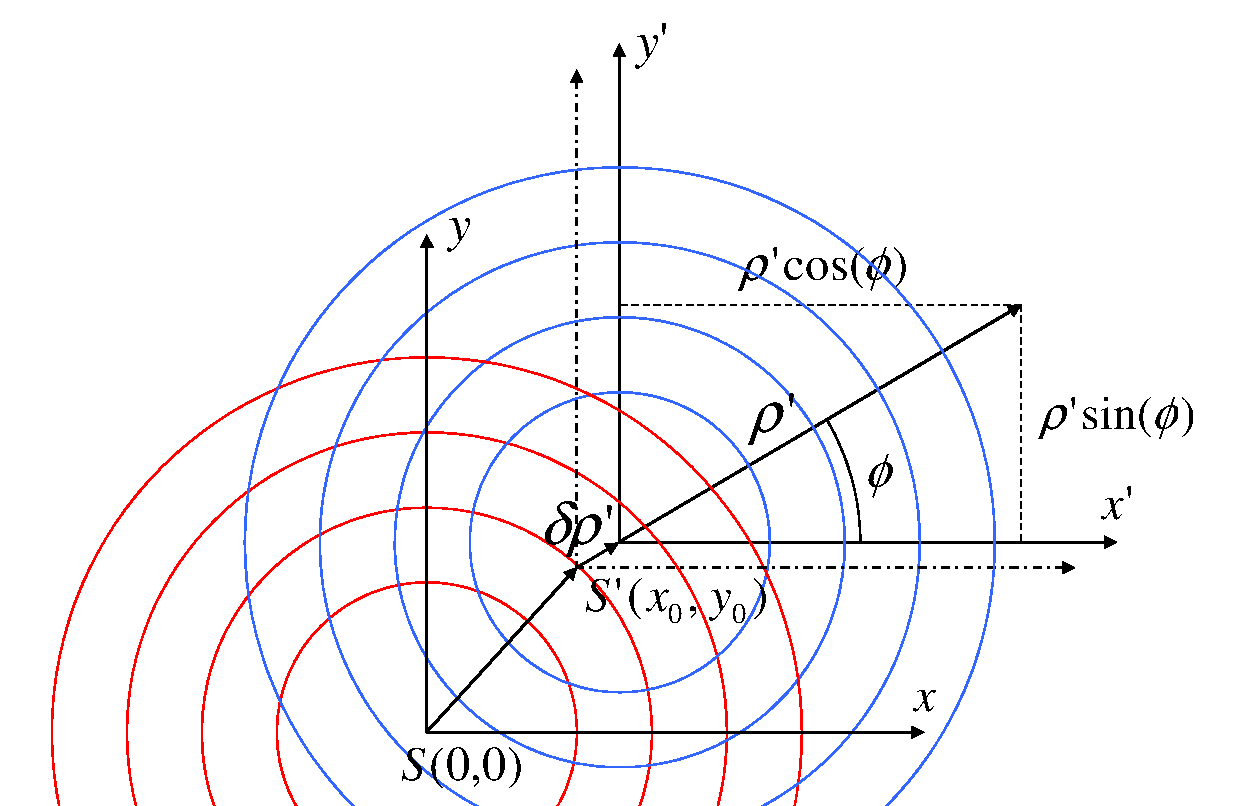
\includegraphics[width=\columnwidth,height=0.4\textheight,keepaspectratio]{map_offset3}%
}
\caption[Illustration of the source of the measured sinusoidal fluctuation in the radial field component]{Illustration of the source of the measured sinusoidal fluctuation in the radial field component.  The mechanical axis $S^\prime$ is offset from the magnetic field axis $S$.  $\delta \rho$ is a linear offset in the measured quantity $\rho$.  Adapted from Refs.~\cite{Lighthall_2008SLM,Vann_2008}.}%
\label{map_off}%
\end{figure}

Using the relationship illustrated in Fig.~\ref{map_off}, the radius relative to the magnetic axis $\rho$ can be written in terms of the measured radius $\rho^\prime$ as
\begin{equation}
\rho=\sqrt{[(\rho^\prime + \delta \rho) \cos(\phi)+x_0]^2+[(\rho^\prime + \delta \rho)\sin(\phi)+y_0]^2}
\label{rho_offset}
\end{equation}
where $x_0$ and $y_0$ are the horizontal and vertical alignment offsets, respectively, and $\delta \rho^\prime$ is a linear offset in $\rho^\prime$.  The linear offset parameter is included because the exact position of the Hall plate sensor within the tip of the probe had to be estimated from non-technical schematics.  All of the readings in the ``axial'' sensor for the measurements at $z= \pm 95$\,cm corresponded to a positive radial flux, except for those at $\rho^\prime=0$, which measured a negative flux.  Therefore, those measurements were actually sampling the field at a radius of $-\delta \rho^\prime$.  Also, since this feature was absent from the measurements at $\rho^\prime \geq 1$\,cm, the value of $\delta \rho^\prime$ must be $< 1$\,cm.

When the HELIOS solenoid was installed on the ATLAS beam line, it was aligned such that the beam path was collinear with the mechanical axis of the solenoid.  Therefore, an offset between the magnetic field axis and the mechanical axis of the solenoid could have an impact on experiments conducted with HELIOS.  To asses any possible offset, the radial field was analyzed at $z= \pm 95$\,cm, where the radial field is strongest.  In order to have a more statistically significant sample, % of the radial field at $z= \pm 95$\,cm,
 the field cross sections at those points included an additional 576 measurements, made at radius intervals of 1\,cm in the range $0<\rho<10$\,cm.  

To fit the data, the measured radius was related to the sample-point radius by Eq.~\ref{rho_offset}.  Then, the sample-point radius $\rho$ was fit with a cubic function.  For measurements made at $\phi \geq 180^\circ$, the measured radius and field were reflected about the origin to ensure a symmetric fit function.  To determine a $\chi^2$ fit value, the average value of the tangential field component (for all measurements) was used as the value of the uncertainty in the magnetic field measurement $\delta \mathscr{B}=15.4$\,G.  The results of fitting the radial field at the given cross sections is shown Table~\ref{offset_param} and Fig.~\ref{cubic_fit}.

\begin{table}
  \begin{center}
    \begin{tabular}{.....|....}
      \hline
      \multicolumn{1}{c}{\multirow{3}{*}{$z$}} &
      \multicolumn{4}{c|}{$\rho^\prime \leq 30$\,cm} &
      \multicolumn{4}{c}{$\rho^\prime \leq 45$\,cm} \\ \cline{2-9}
       &\multicolumn{1}{c}{$x_0$} &\multicolumn{1}{c}{$y_0$} &\multicolumn{1}{c}{ $\delta \rho^\prime$}&\multicolumn{1}{c|}{$\chi^2/\mathrm{dof}$}
              &\multicolumn{1}{c}{$x_0$} &\multicolumn{1}{c}{$y_0$} &\multicolumn{1}{c}{ $\delta \rho^\prime$}&\multicolumn{1}{c}{$\chi^2/\mathrm{dof}$}\\\hline \hline 
       %& $x_0$ & $y_0$ & $\delta \rho^\prime$&$X^2/\mathrm{dof}$\\\hline \hline 
      -95.85&0.26&4.30&-0.08&5.19&0.35&4.95&2.77&109.8\\
      +94.15&-0.22&-1.59&0.26&1.38&0.01&1.45&2.51&75.7\\
      \multicolumn{1}{c}{Average}& 0.02 &2.71&0.09&&0.18&3.20&2.64\\\hline
    \end{tabular}
    \label{offset_param}
    \caption[Offset parameters for two different cubic fits to the radial field at $z= \pm 95$\,cm]{Offset parameters for two different cubic fits to the radial field at $z= \pm 95$\,cm.  Values are given in mm.  For both fit ranges $x_0$ is consistent with zero and $\delta \rho^\prime$ is consistent with the required range of 0--10\,mm.}
  \end{center}
\end{table}

\begin{figure}%
\centering
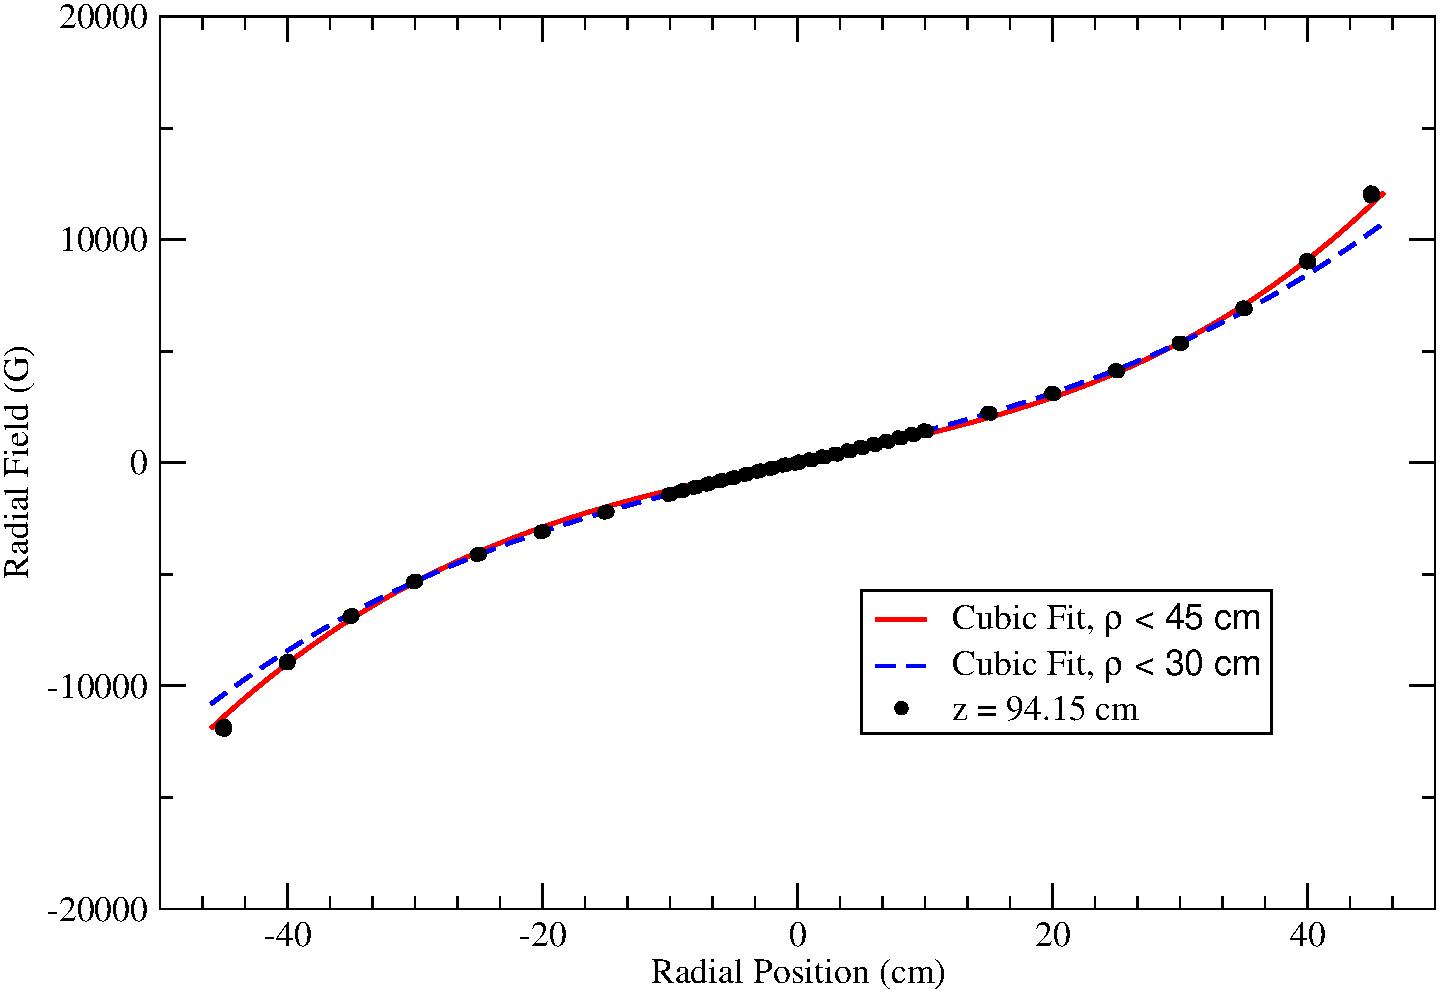
\includegraphics[width=\columnwidth]{cubic_fit2}%
\caption{Radial field data for the $z=94.15$\,cm field cross section measurement with two cubic fits.}%
\label{cubic_fit}%
\end{figure}

The fits indicate that $x_0\approx0$\,mm and $y_0\approx3\,$mm.  This may represent an actual offset in the mechanical structure of the solenoid.  However, the magnitude of the fitted value of $y_0$ is greater for the measurement at $z=-95$\,cm.  This measurement point was nearly 1\,m away from the point where the probe jig was suspended.  It is possible that despite the reinforcement from the trusses, the axial rails of the probe jig were sagging and this is the cause of the vertical offset.  The effect of a genuine mechanical offset is discussed in Chapt.~\ref{simulation}.  Finally, the linear offset is in the range $0<\delta \rho^\prime<1$\,cm, as required by the flux inversion present only in the measurements at $\rho^\prime = 0$.

%Since the bore of the solenoid---and presumably, the solenoid itself---are circular, an asymmetric 
Accounting for the eccentric rotation of the rotation of the probe jig effectively eliminates the azimuthal dependence of the radial field component for smaller radii ($\rho^\prime \leq 30$\,cm).  For larger radii, this correction still leaves a residual variation.  However, the residual azimuthal variations in the radial field components are on the order of 0.5\%, and scales roughly with the axial field component, which is consistent with a trivial non-perpendicularity of the Hall plate sensors.

\subsection{Determining the Absolute Field}
\label{absf}
The field mapping was conducted with a current of 363.00\,A in the solenoid coils.  This value was chosen to achieve a 2.00\,T field based on the field-to-current ratio given in the solenoid service manual as shown in Table~\ref{current}.  A field of 2\,T (20,000\,G) was selected in order to comply with safety guidelines, specifically, the whole body exposure ceiling limit value (TLV-C) as suggested by the American Conference of Governmental Industrial Hygienists (ACGIH).  However, the initial result of the field mapping indicated a central field of 1.9159\,T.  This measured value corresponds to a different field-to-current ratio, as shown in Table~\ref{current}.

\begin{table*}
\begin{center}
\begin{tabular}{rccc.}
\hline
Source&$\mathscr{B}_0$ Field (g)&Current (A)& Ratio (g/A)&
\multicolumn{1}{c}{Slope (keV/mm)}\\\hline \hline
Service Manual&30000&543.96&55.15&10.124\\
Field Map&19159&363.00&52.78&9.698\\\hline
\end{tabular}
\label{current}
\caption[Field-to-current relations for the HELIOS solenoid]{Field-to-current relations for the HELIOS solenoid.  Values are based on the magnet specifications given in the solenoid service manual and the results of the field map.  Also shown is the expected slope of the kinematic loci from the $d$($^{28}$Si,$p$)$^{29}$Si reaction.}
\end{center}
\end{table*}

This discrepancy introduces a dilemma: either the solenoid's field response is nonlinear or the field mapping measurements are systematically inaccurate.  To address this issue, the magnetic field was measured by a one-dimensional Hall probe at a fixed representative point on the flange face during the process of energizing the solenoid. The results of this measurement are shown in Fig.~\ref{field_lin}.  It is clear from this figure that the field response is indeed linear with current.  However, it is also clear from the self-consistent nature of the field mapping data that whatever systematic error is present effects all of the data points equally.  The conclusion is then that the measured field map quantities are 95.8\% of the actual value.

\begin{figure}[t]
\centering
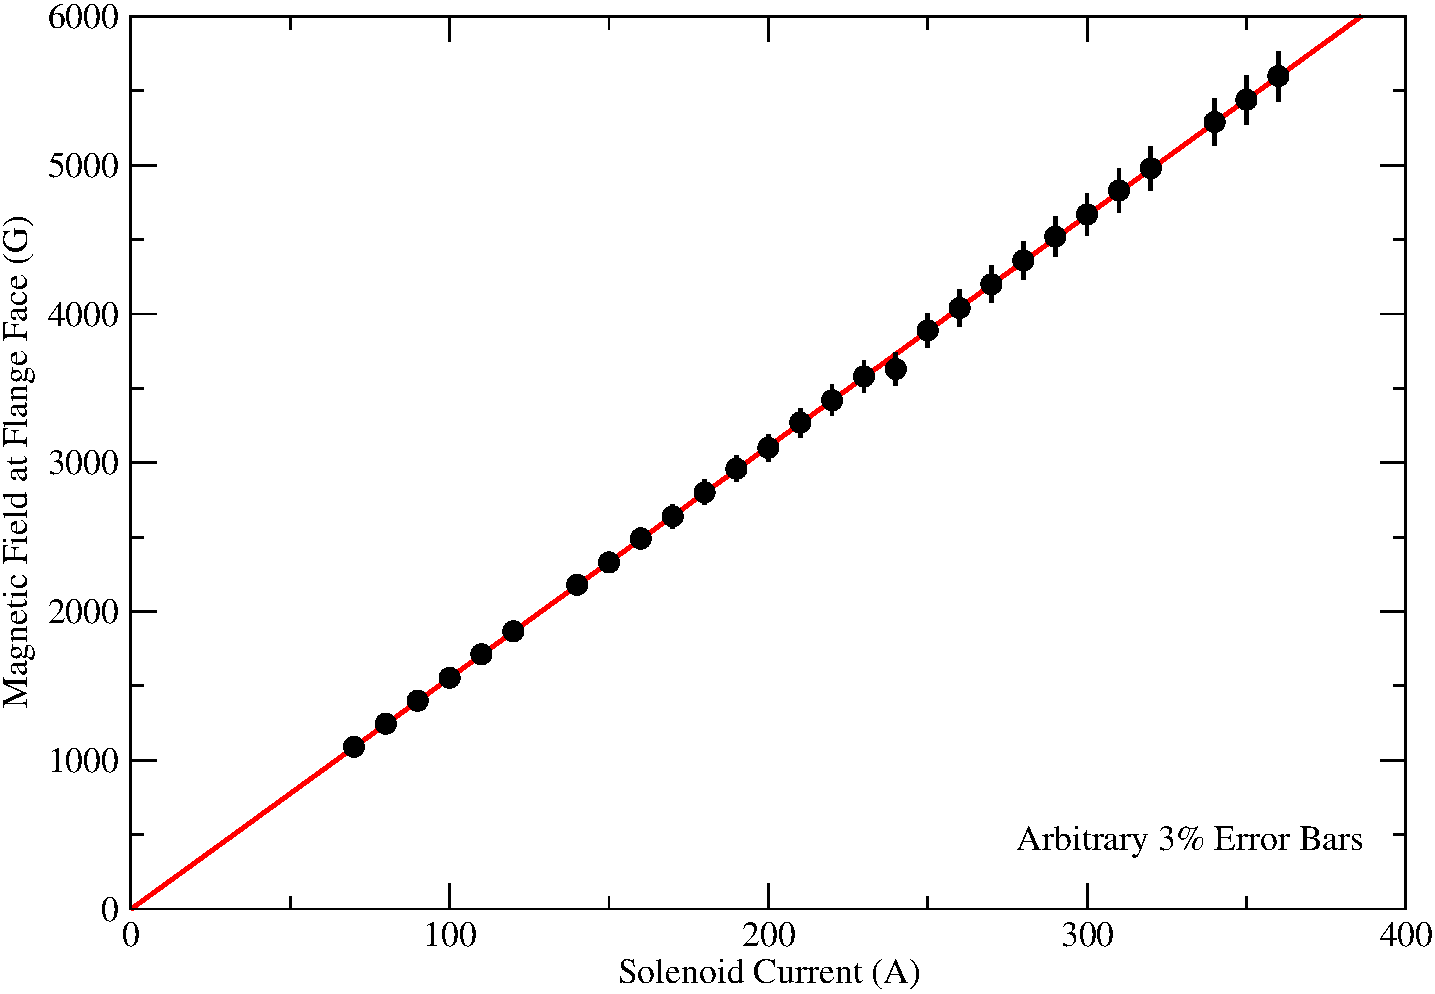
\includegraphics[keepaspectratio,height=0.5\textheight,width=\columnwidth]{Field_Linearity}%
\caption[Field linearity as measured during a solenoid-energizing procedure]{Field linearity as measured during a solenoid-energizing procedure.  Measurements were made at the flange face of the HELIOS solenoid during a ramp-up to 363\,A.  The red line is a linear regression fit to the data.}%
\label{field_lin}%
\end{figure}

This conclusion is further supported by an analysis of the data from the first reaction measured with HELIOS.  For a given reaction and bombarding energy, Eq.~\ref{slope_calc} gives the expected slope of the kinematic loci based on the (uniform) magnetic field.  Fig.~\ref{badslope} shows data from three different position settings that have been shifted to line up with calculations for the two possible field strengths.  The calculations for $\mathscr{B}_0=1.91$\,T clearly do not line up with the data, while the calculations for $\mathscr{B}_0=2.00$\,T are in good agreement.

An additional implication of understanding the field-to-current ratio of the HELIOS solenoid is the maximum field setting.  The HELIOS solenoid is rated as a 3.0\,T magnet; this field value is achieved with a solenoid current of 543.96\,A, as shown in Table~\ref{current}.  However, the Siemens Model 3600 Magnet Power Supply used to energize the HELIOS solenoid will only output 518.00\,A to the solenoid.  This corresponds to a maximum possible central field value for the HELIOS solenoid of 2.8568\,T.\footnote{The value reported in Ref.~\cite{Schiffer_2010} (2.7\,T) is off by a factor of 95.8\%, which is the value based on the field map.}  This maximum field value corresponds to  a length parameter of $\mathscr{B}\rho=1.32$\,T$\cdot$m and a radial parameter of $\mathscr{B}L=6.70$\,T$\cdot$m, exceeding the requirements put forth in Ref.~\cite{Wuosmaa_2007}.

\begin{figure}%
\centering
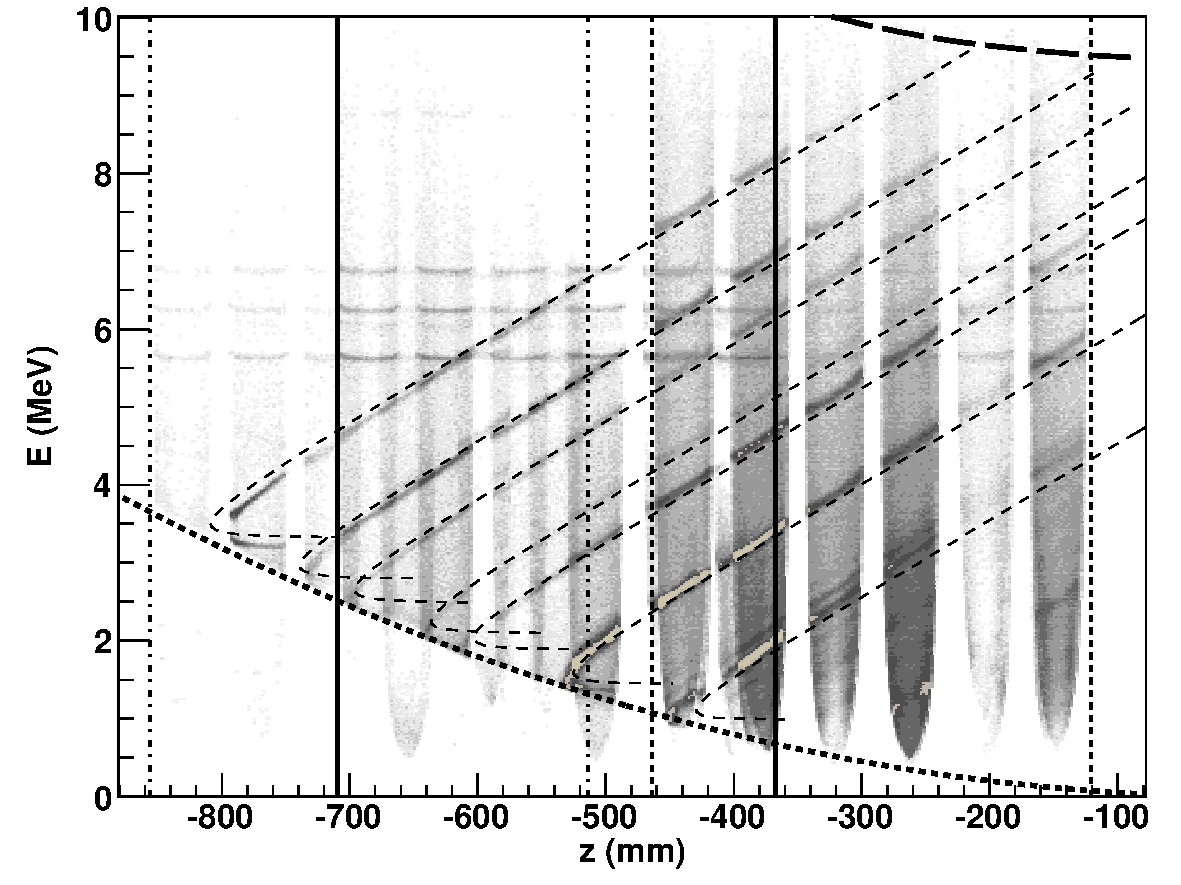
\includegraphics[width=\columnwidth,height=0.4\textheight,keepaspectratio]{cShift_191_bw}\\
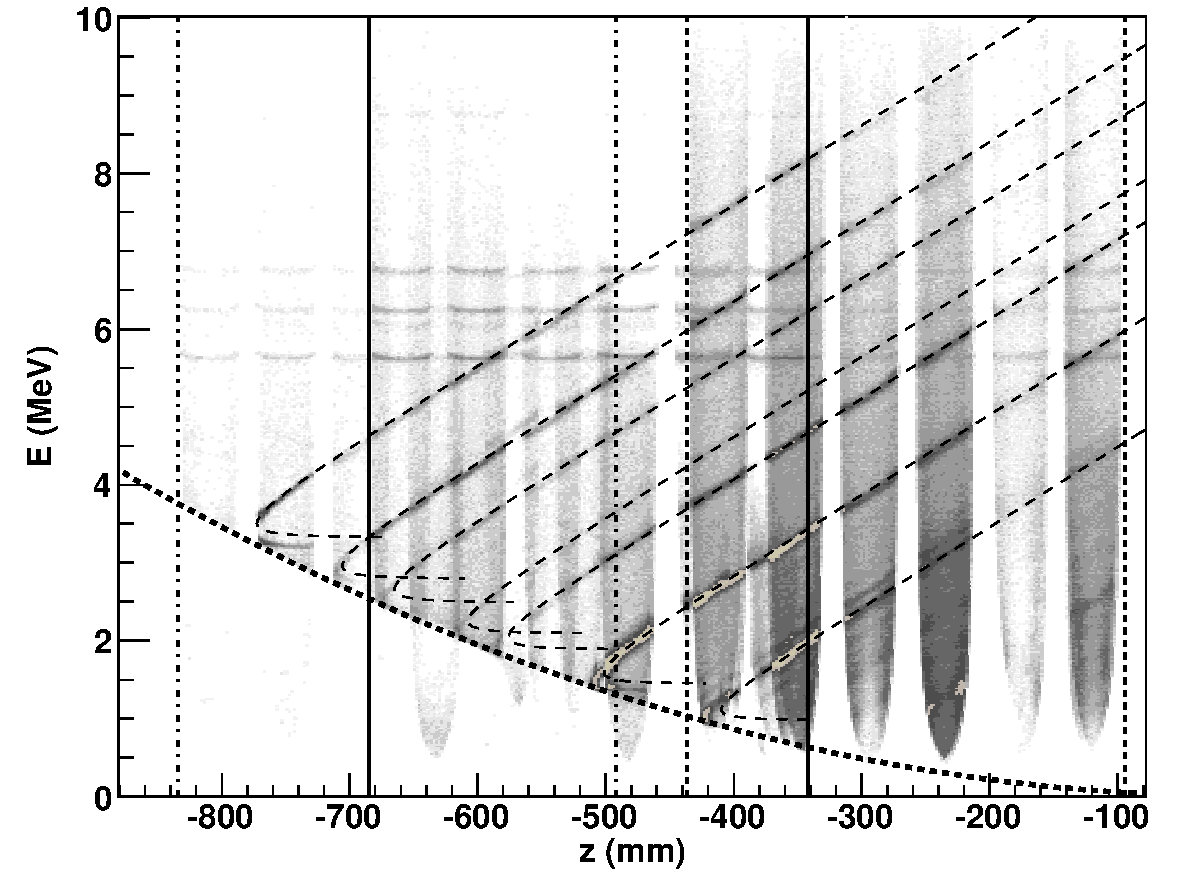
\includegraphics[width=\columnwidth,height=0.4\textheight,keepaspectratio]{cShift_200_bw}%
\caption[Determination of the absolute field by slope analysis]{Determination of the absolute field by slope analysis.  Calculated proton energies (fine dashed lines) are overlaid on two analyses of the same data set.  The data have been shifted in $z$ to best fit the calculations for $\mathscr{B}_0=1.91$\,T (top) and $\mathscr{B}_0=2.00$\,T (bottom).  In the top figure, note that the calculations overestimate $E_\mathrm{lab}$ at low energy and underestimate $E_\mathrm{lab}$ at high energy, indicating a mis-match in slope ($\mathscr{B}$-field).  In the lower figure, the data and calculations are aligned, supporting the conclusion that the field strength was indeed $\mathscr{B}_0=2.00$\,T.  In each panel, pairs of vertical lines indicate detector positions and bold dashed curves indicate the (calculated) acceptance limits.  The upper limit occurs above the axis limit in the lower figure.}%
\label{badslope}%
\end{figure}